\documentclass[]{IAC_style}

\begin{document}

\IACpaperyear{2024} % format yyyy
\IACpapernumber{IAC-2x-XX-XX-X-xXXXXX} % full paper id
\IAClocation{Milan, Italy} % used in the header
\IACdate{14-18 October 2024} % used in the header

% Which copyright? If B, put the copyright holder.
%\IACcopyrightA{}
\IACcopyrightB{'copyright holder'}

\title{Example of IAC template}

%\IACauthor{Author name}{corresponding affiliation: nr. of corresponding affiliation}{is corresponding author? 0-1}
\IACauthor{Davide Grande$^{\orcidlink{0000-0000-0000-0000}}$}{1}{1}
\IACauthor{Stefano Farì$^{\orcidlink{0000-0000-0000-0000}}$}{2}{0}

% Input affiliations here, order is relevant
\IACauthoraffiliation{Lorem Ipsum1. Sed ut perspiciatis unde omnis iste natus error sit voluptatem accusantium doloremque laudantium \normalfont{E-mail:~\authormail{my.email@email.com}}}
\IACauthoraffiliation{Lorem Ipsum2. Sed ut perspiciatis unde omnis iste natus error sit voluptatem accusantium doloremque laudantium \normalfont{E-mail:~\authormail{my.email@email.com}}}

\abstract{
A concise and factual abstract (written in third person and in one paragraph) of no more than 400 words is required. The abstract should state briefly the purpose of the research, the principal results and major conclusions. An abstract must be stand alone and complete in itself with no references to the main body of the manuscript. References should be avoided, but if essential, then cite the author(s) and year(s). Also, non-standard or uncommon abbreviations should be avoided, but if essential they must be defined at their first mention in the abstract itself. Readers should not have to read the full text to understand the abstract. The abstract can be an updated version of the one submitted at the call-for-abstracts, but its contents must not differ substantially.
}


\maketitle
\thispagestyle{fancy} % resets proper header/footer

\section*{Nomenclature}
This section is not numbered. A nomenclature section could be provided when there are mathematical symbols in your paper. Superscripts and subscripts must be listed separately. Nomenclature definitions should not appear again in the text.

\section*{Acronyms/Abbreviations}
This section is not numbered. Define acronyms and abbreviations that are not standard in this section. Such acronyms and abbreviations that are unavoidable in the abstract must be defined at their first mention there. Ensure consistency of abbreviations throughout the article. Always use the full title followed by the acronym (abbreviation) to be used, e.g., reusable suborbital launch vehicle (RSLV), International Space Station (ISS).


\section{Introduction}
Section headings are in bold and placed flush on the left hand margin of the column.
The Introduction Section is to state the objectives of the work, provide an adequate background including a brief literature survey, major differences from the others, and sectional organization of this paper. Avoid a too detailed and lengthy literature survey and a summary of the results.
Divide your paper into clearly defined and numbered sections numbered 1., 2., ...~. Subsections should be numbered 1.1 (then 1.1.1, 1.1.2, ...), 1.2, etc. Use this numbering also for internal cross-referencing: do not just refer to “the text”. Any subsection may be given a brief heading. Each heading should appear on its own separate line.

Indicate references by number(s) in square brackets in line with the text. The actual authors can be referred to, but the reference number(s) must always be given.
Ex. \cite{chang2015space}, \cite{van2010art}, \cite{mettam2009chapter,strunk2000elements} or \cite{mettam2009chapter,strunk2000elements,mack2015virgin}.

\subsection{Subsection headings}
Subsection headings are in italics and placed flush on the left hand margin of the column.

\subsubsection{Sub-subsection headings}
Sub-subsection headings are in italics and placed flush on the left hand margin of the column.

\section{Material and methods}
Provide sufficient detail to allow the work to be reproduced. Methods already published should be indicated by a reference: only relevant modifications should be described.

\section{Theory and calculation}
A Theory section should extend, not repeat, the background to the article already dealt with in the Introduction and lay the foundation for further work. In contrast, a Calculation section represents a practical development from a theoretical basis.

\subsection{Equation numbers}
Number consecutively any equations that have to be displayed separately from the text (if referred to explicitly in the text). The numbers identifying the equations should be placed in parentheses to the right of the equation. For example:

\begin{equation}
\vec{F}_g = -G \frac{m \times m_E}{R_E^2} \vec{i}_r = m \vec{g}_{ta}
\end{equation}

\subsection{Figure numbers}
Ensure that each figure/illustration has a title. All figures/illustrations must be numbered and cited (see Fig. 1) in the text consecutively. Place figures/ illustrations as close as possible to the first references to them in the manuscript. Restrict them to single-column width unless this would make them illegible (then extend these figures/illustrations across two columns or place them to the end of your paper).

\begin{figure}[H]
\centering
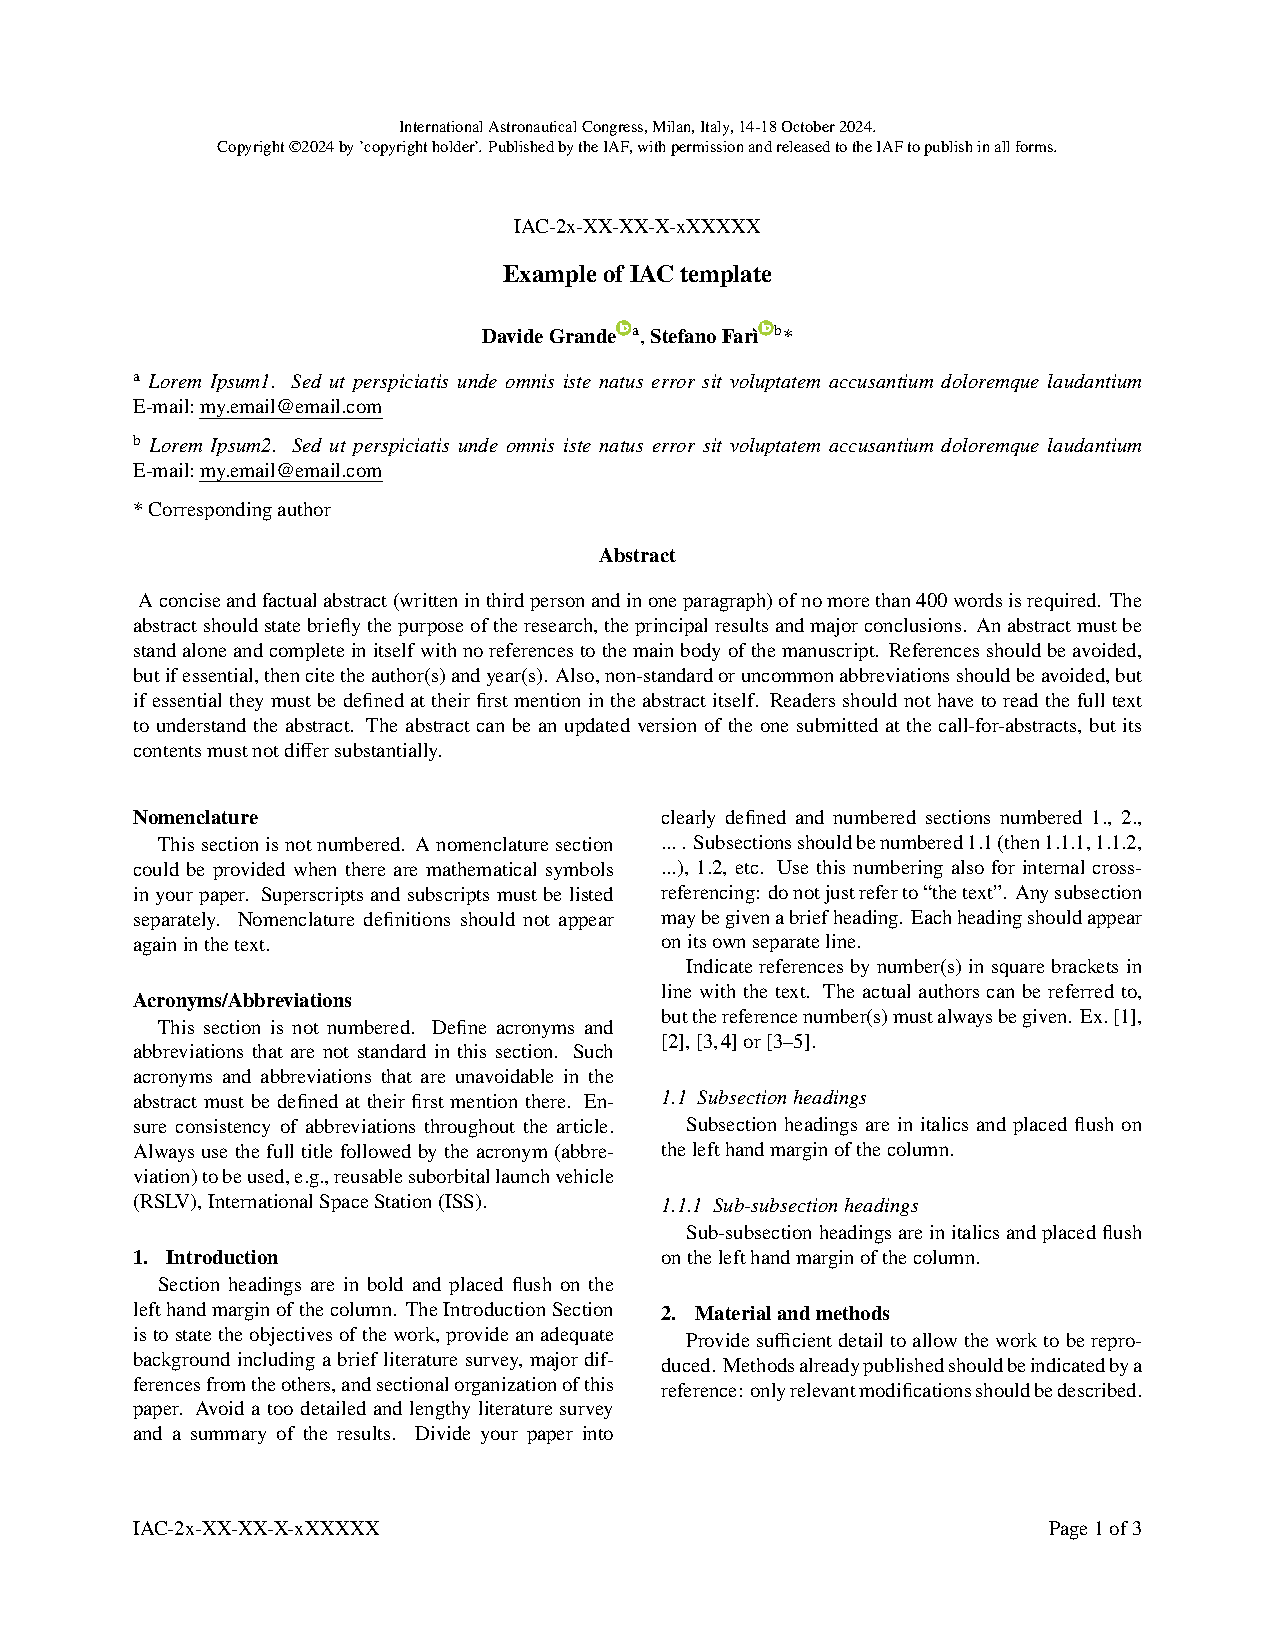
\includegraphics[width=\columnwidth]{pics/example.jpg}
\label{fig:example}
\caption{SpaceShipTwo carried under White Knight Two.}
\end{figure}

\subsection{Tables}
Tables can be placed either next to the relevant text in the article, or on separate page(s) at the end. Number and cite (as shown in Table 1) tables consecutively in accordance with their appearance in the text. Place table title above and any remarks below the table body.

\newcolumntype{b}{X}
\newcolumntype{s}{>{\hsize=.5\hsize}X}
\begin{table}
\centering
\label{tab:table}
\caption{Major data of the orbits of Venus, Earth, Mars and Jupiter.}
\begin{tabularx}{\columnwidth}{bssss}
\hline
& Venus & Earth & Mars & Jupiter\\\hline
M/ME & 0.82 & 1 & 0.11 & 317.89\\
e & 0.007 & 0.017 & 0.093 & 0.048\\
R (AU*) & 0.7233 & 1 & 1.524 & 5.203\\
i (deg) & 3.40 & 0 & 1.85 & 1.30\\
T (years) & 0.62 & 1 & 1.88 & 11.86\\
\hline
\end{tabularx}
\\\footnotesize{* AU = Astronomical Unit}
\end{table}


Tables with a moderate amount of information should be positioned within one column. Tables, figures or pictures with large amounts of information or size may extend across two columns.


\subsection{Page Numbers}
Indicate page number at the bottom of each page.

\section{Results}
Results should be clear and concise.


\section{Discussion}
This should explore the significance of the results of the work, not repeat them. A combined Results and Discussion section is often appropriate. Avoid extensive citations and discussion of published literature.

\section{Conclusions}
The main conclusions of the study may be presented in a short Conclusions section, which may stand alone or form a subsection of a Discussion or Results and Discussion section.

\section*{Acknowledgements}
This section is not numbered.


\begin{appendices}
\section{My title}
This section is not numbered. Figures and equations numbering slightly change:
\begin{equation}
F = ma
\end{equation}


\section{My title}
This section is not numbered.
\end{appendices}

\bibliographystyle{unsrt}
\bibliography{biblio}

%\custombibliography{biblio}  % This is the .bib file containing your bibliography data


\end{document}